\documentclass[12pt,a4paper]{article}
\usepackage{microtype}
\usepackage{lmodern}
\usepackage{mathpazo}
\usepackage{tabularx}
\usepackage{minted}
\usepackage{latexsym}
\usepackage{longtable}
\usepackage{amsmath,amssymb,amsthm}
\usepackage[english]{babel}
\usepackage{float}
\usepackage{graphicx}
\usepackage{hyperref}
\usepackage[utf8]{inputenc}
\usepackage{listings}
\usepackage{xcolor}
\usepackage{array}

% use more of the page
\usepackage[scale=0.8]{geometry}
% do not move figures across sections
\usepackage[section]{placeins}

\usepackage{graphicx} % Required for inserting 
\usepackage{parskip}
\usepackage{amsfonts}
\usepackage{xurl}
\usepackage[colorinlistoftodos]{todonotes}
\usepackage{caption}
\usepackage{subcaption}

% Sensible defaults for lstlistings
\lstset{
  basicstyle=\footnotesize\ttfamily,
  belowcaptionskip=1\baselineskip,
  breaklines=true,
  commentstyle=\bfseries\color{purple!40!black}
  frame=L,
  identifierstyle=\color{blue},
  keywordstyle=\bfseries\color{green!40!black},
  language=python,
  showstringspaces=false,
  stringstyle=\color{orange},
  xleftmargin=\parindent,
}
% prettier links
\hypersetup{
colorlinks,
linkcolor={red!50!black},
citecolor={blue!50!black},
urlcolor={blue!80!black}
}
\urlstyle{rm}

\begin{document}
\title{Advanced Deep Learning 2024\\Assignment 1}
\author{Johannes Sindlinger, Christoph Kern, Amos Weckström}
\maketitle

\section{Deep versus wide networks}
\begin{figure}
  \begin{center}
%    \includegraphics[width=.75\textwidth]{Assignment1_Question6_Plot1}
  \end{center}
  \caption{Every figure and table has a caption and is referred to 
    in the text body.\label{fig:q6p1}}
\end{figure}

You can add code like this
\begin{lstlisting}
c = conv(x)
c = torch.square(c)
\end{lstlisting}

For combining the filter outputs, you can  use 
\lstinline{torch.sum}, but you have to set the \lstinline{axis}
argument properly.
\section{Convolutional neural networks}

no problem if you do or do not see the activation function when you output of the architecture 


\subsection{Basic CNN definition}
\subsection{Activation function before or after pooling?}
\subsection{Data augmentation}
\subsection{Batch normalization}
\subsection{Experimental architecture comparison}
\section{Fully convolutional neural networks}
\subsection{Receptive field and double convolution}


\begin{center}
\begin{tabular}{lcccc}
     &  $d=1$ &  $d=2$ &  $d=3$ & general $d$\\
 number of trainable parameters   &$n$& $n^2$& $n^3$ & $n^d$\\
 receptive field size  &$n$& $n^2$& $n^3$ & $n^d$
\end{tabular}
    \end{center}
\section{U-Nets and MLOps}
\subsection*{Subtask 1}

Aside from regulating the imports and setting the device (gpu, cpu) to run the tensor operations on, the notebook has the following components:

\footnotesize
\begin{longtable}{|m{0.5\textwidth}|m{0.43\textwidth}|} \hline
\textbf{Code Snippet} & \textbf{Description} \\ \hline
\begin{lstlisting}
def load_npz_dataset(path, keys=('x_train', 'y_train', 'x_val', 'y_val', 'x_test', 'y_test')):
    archive = np.load(path)
    return [archive.get(key) for key in keys]

def as_torch_dataset(x_arr, y_arr):
    dataset = torch.utils.data.TensorDataset(
        torch.FloatTensor(x_arr),
        torch.FloatTensor(y_arr)
    )
    return dataset
\end{lstlisting} & \lstinline|load_npz_dataset| loads a NPZ-file from the given path and returns, by default, lists representing the training, validation and test sets.\vspace{8px}

\lstinline|as_torch_dataset| takes the data values and their corresponding labels and converts them to a \lstinline|TensorDataset|.
\\ \hline
\begin{lstlisting}
def plot_image_with_segmentation(image, segmentation, ax=None):
    ...
    im = image.cpu().detach().numpy()
    segm = segmentation.cpu().detach().numpy()
    ax.imshow(im.squeeze(), cmap="gray")
    mask = segm < 0.5
    ax.imshow(mask.squeeze(), cmap="Set1", alpha=0.5)
    return plt.gcf(), ax
\end{lstlisting} & This function takes an image and draws an overlay representing the segmentation on top of the image. The threshold for any pixel to be colored is 0.5. Optionally, a x- and y-axis plus a title may be added to the graphic.
\\ \hline
\begin{lstlisting}
def evaluate_model_on_single_image(model, x, device=device):
    with torch.no_grad():
        x = x.to(device)
        return model(x.view(1, *x.shape))
        
def evaluate_model(model, data_loader, metrics_dict, reduction=True, device=device):
    metrics = defaultdict(list)
    with torch.no_grad():
        for i, (batch_x, batch_y) in enumerate(data_loader):
           ...
\end{lstlisting} & \lstinline|evaluate_model_on_single_image| predicts the segmentation for a single image using the given model. \vspace{8px}

\lstinline|evaluate_model| is similar, but instead of taking just one image, it predicts on batches of images provided by \lstinline|data_loader|. Furthermore, one can choose a set of metrics to determine based on the results, either for each image or the mean over all of them. 
\\ \hline 
\begin{lstlisting}
def save_model(model, path, optimizer=None):
    ...
    torch.save(state, path)


def load_model(model, path, optimizer=None):
    state = torch.load(path)
    ...
\end{lstlisting} & Saves/loads the state of the model to/from a given path. Optionally, one can also save/load the state of the optimizer. 
\\ \hline 
\begin{lstlisting}
def plot_histories(train_history=None, val_history=None, label="Loss"):
...
    if train_history:
        ax.plot(epochs, train_history, label="Training", color="black")
    if val_history:
        ax.plot(epochs, val_history, label="Validation", color="darkred")
...
\end{lstlisting} & The function takes a list of training and/or validation metrics (e.g. Loss, F1 score) and plots them versus number of epochs.
\\ \hline 
\begin{lstlisting}
def run_one_epoch(model, loss, optimizer, train_loader, val_loader, n_epochs, metrics_dict, epoch, device=device):
    train_losses = []
    for i, (batch_x, batch_y) in enumerate(train_loader):
...
        logits = model(batch_x)

        loss_tensor = loss(logits, batch_y)
...

    val_metrics = evaluate_model(
        model=model,
        data_loader=val_loader,
        metrics_dict=metrics_dict
    )
    return {"loss": np.mean(train_losses)}, val_metrics
\end{lstlisting} & This function does a forward pass through the network (\lstinline|model|) for each batch provided by the \lstinline|train_loader|, computes the loss using the provided loss function, determines the gradients based on the loss, and uses the provided optimizer to adjust the weights and biases within the network. At the end of this epoch, the model is validated using the data provided by the \lstinline|val_loader| and a set of chosen metrics is computed. 
\\ \hline 
\begin{lstlisting}
def merge_list_of_dicts(list_of_dicts):
    merged = defaultdict(list)
...


def training_loop(model, loss, optimizer, train_loader, val_loader, n_epochs, init_epoch=None, metrics_dict=None, save_path=None):
...
    try:
        for i in range(init_epoch, n_epochs):
            train_metrics, val_metrics = run_one_epoch(...)
...
\end{lstlisting} & \lstinline|merge_list_of_dicts| takes a list of dictionaries and merges them into one dictionary pointing to lists. This is used by \lstinline|training_loop| to merge the training and validation history, respectively. \vspace{8px}

\lstinline|training_loop| is the main entry point to train the model, running \lstinline|run_one_epoch| for the number of given epochs. The function keeps track of the metrics computed for each epoch in order to provide a history of the metrics. Furthermore, it can save the learning progress after the completion of an epoch. 
\\ \hline 
\begin{lstlisting}
data_root='./datasets'
data_npz='lung_field_dataset.npz'
...
x_train, y_train, x_val, y_val, x_test, y_test = load_npz_dataset(data_fn)
...
train_dataset = as_torch_dataset(x_train, y_train)
val_dataset = as_torch_dataset(x_val, y_val)
test_dataset = as_torch_dataset(x_test, y_test)

train_loader = torch.utils.data.DataLoader(train_dataset, batch_size=16, shuffle=True)
...
\end{lstlisting} & This section of the script loads the dataset using the previously defined \lstinline|load_npz_dataset| function, and converts the training, validation, and test data points and labels into corresponding torch datasets using the previously defined \lstinline|as_torch_dataset| function. Finally, these datasets are brought into a data loader with a defined batch size. As an example, the first image of the training data set is plotted with the previous defined \lstinline|plot_image_with_segmentation| function.
\\ \hline
\begin{lstlisting}
model = smp.Unet(encoder_name='efficientnet-b0',in_channels=1,classes=1)
model.to(device)
optimizer = torch.optim.Adam(model.parameters(), lr=0.0001)
\end{lstlisting} & This creates a U-Net model instance provided by the smp framework, a neural network commonly used for image segmentation tasks. Furthermore, an Adam-optimizer is defined to update the weights and biases of the U-Net model during training. 
\\ \hline
\begin{lstlisting}
init_epoch = None
if init_epoch != None:
    load_model(model, f"epoch_{init_epoch}_model.ckpt", optimizer)
\end{lstlisting} & These lines load a model from the directory for a given epoch (set by \lstinline|init_epoch|) that has previously been saved during the learning process in order to be able to continue training.
\\ \hline
\begin{lstlisting}
loss = torch.nn.MSELoss(reduction="mean")
metrics = {"f1": torchmetrics.classification.F1Score(task='binary', num_classes=1, average="macro")}

train_history, val_history = training_loop(
    model=model,
    loss=loss,
    optimizer=optimizer,
    train_loader=train_loader,
    val_loader=val_loader,
    init_epoch=init_epoch,
    n_epochs=100,
    metrics_dict=metrics,
    save_path="model.ckpt"
)
\end{lstlisting} & This function starts the learning process, using the mean squared error for the loss and the previously defined training/validation data and optimizer. The training process will go over 100 epochs, and we additionally compute the macro-averaged F1 score as a metric. 
\\ \hline
\begin{lstlisting}
plot_histories(train_history['loss'], val_history['loss'], label="Loss")
plot_histories(train_history=None, val_history=val_history['f1'], label="F1 Score")
plt.show()
\end{lstlisting} & These lines plot the history of the loss during training and validation, as well as a plot of the F1 score produced during validation. This uses the previously defined \lstinline|plot_histories| function.
\\ \hline
\begin{lstlisting}
x,y = test_dataset[0]
pred = evaluate_model_on_single_image(model, x)
...
plot_image_with_segmentation(x, y, ax=ax1)
plot_image_with_segmentation(x, pred, ax=ax2)
plt.show()
\end{lstlisting} & These lines run the previously defined \lstinline|evaluate_model_on_single_image| function on the first instance of the test dataset and our trained model and draws the predicated segmentation together with the actual segmentation using the \lstinline|plot_image_with_segmentation| function. 
\\ \hline
\begin{lstlisting}
f1_test_scores = evaluate_model(model, test_loader, metrics, reduction=False)["f1"]

print("Test cases:", len(f1_test_scores))
print("Mean F1:   ", np.mean(f1_test_scores))
print("STD  F1:   ", np.std(f1_test_scores))
print("Min. F1:   ", np.min(f1_test_scores))

sum(p.numel() for p in model.parameters())
\end{lstlisting} & Finally, at the end we use \lstinline|evaluate_model| to compute the F1 score on the test data using the trained model, and then we calculate the mean, standard deviation and the minimum F1 score over the results. Also, we calculate the size of the model based on the number of parameters. 
\\ \hline
\end{longtable}
\normalsize
\subsection*{Subtask 2}

In order to log data during the training process, we add the following line of code inside the for-loop of the \lstinline|training_loop| function, right after calling \lstinline|run_one_epoch|:
\begin{lstlisting}
wandb.log({**train_metrics, **val_metrics})
\end{lstlisting}
This logs all training metrics and validation metrics for each epoch. The training metrics include the mean loss for each epoch. The validation metrics are chosen by the caller of the function. For instance, in the current code, the F1 score is computed.

Additionally, before running the \lstinline|training_loop| in our code, we add the following lines of code to initialize the logging process with W\&B for the current run and tells W\&B the configuration that is currently used.
\begin{lstlisting}
run = wandb.init(project='x_ray_segmentation_erda')

config = wandb.config
config.batch_size = 16
config.epochs = 100
config.learning_rate = 0.0001
config.optimizer = "adam"
\end{lstlisting}
Running the code will start the learning process and will send the logged data to W\&B. W\&B then produces following graphs presented in Figure~\ref{fig:loss}. 

\begin{figure}[!htb]
    \centering
    \begin{subfigure}[b]{0.49\textwidth}
        \centering
        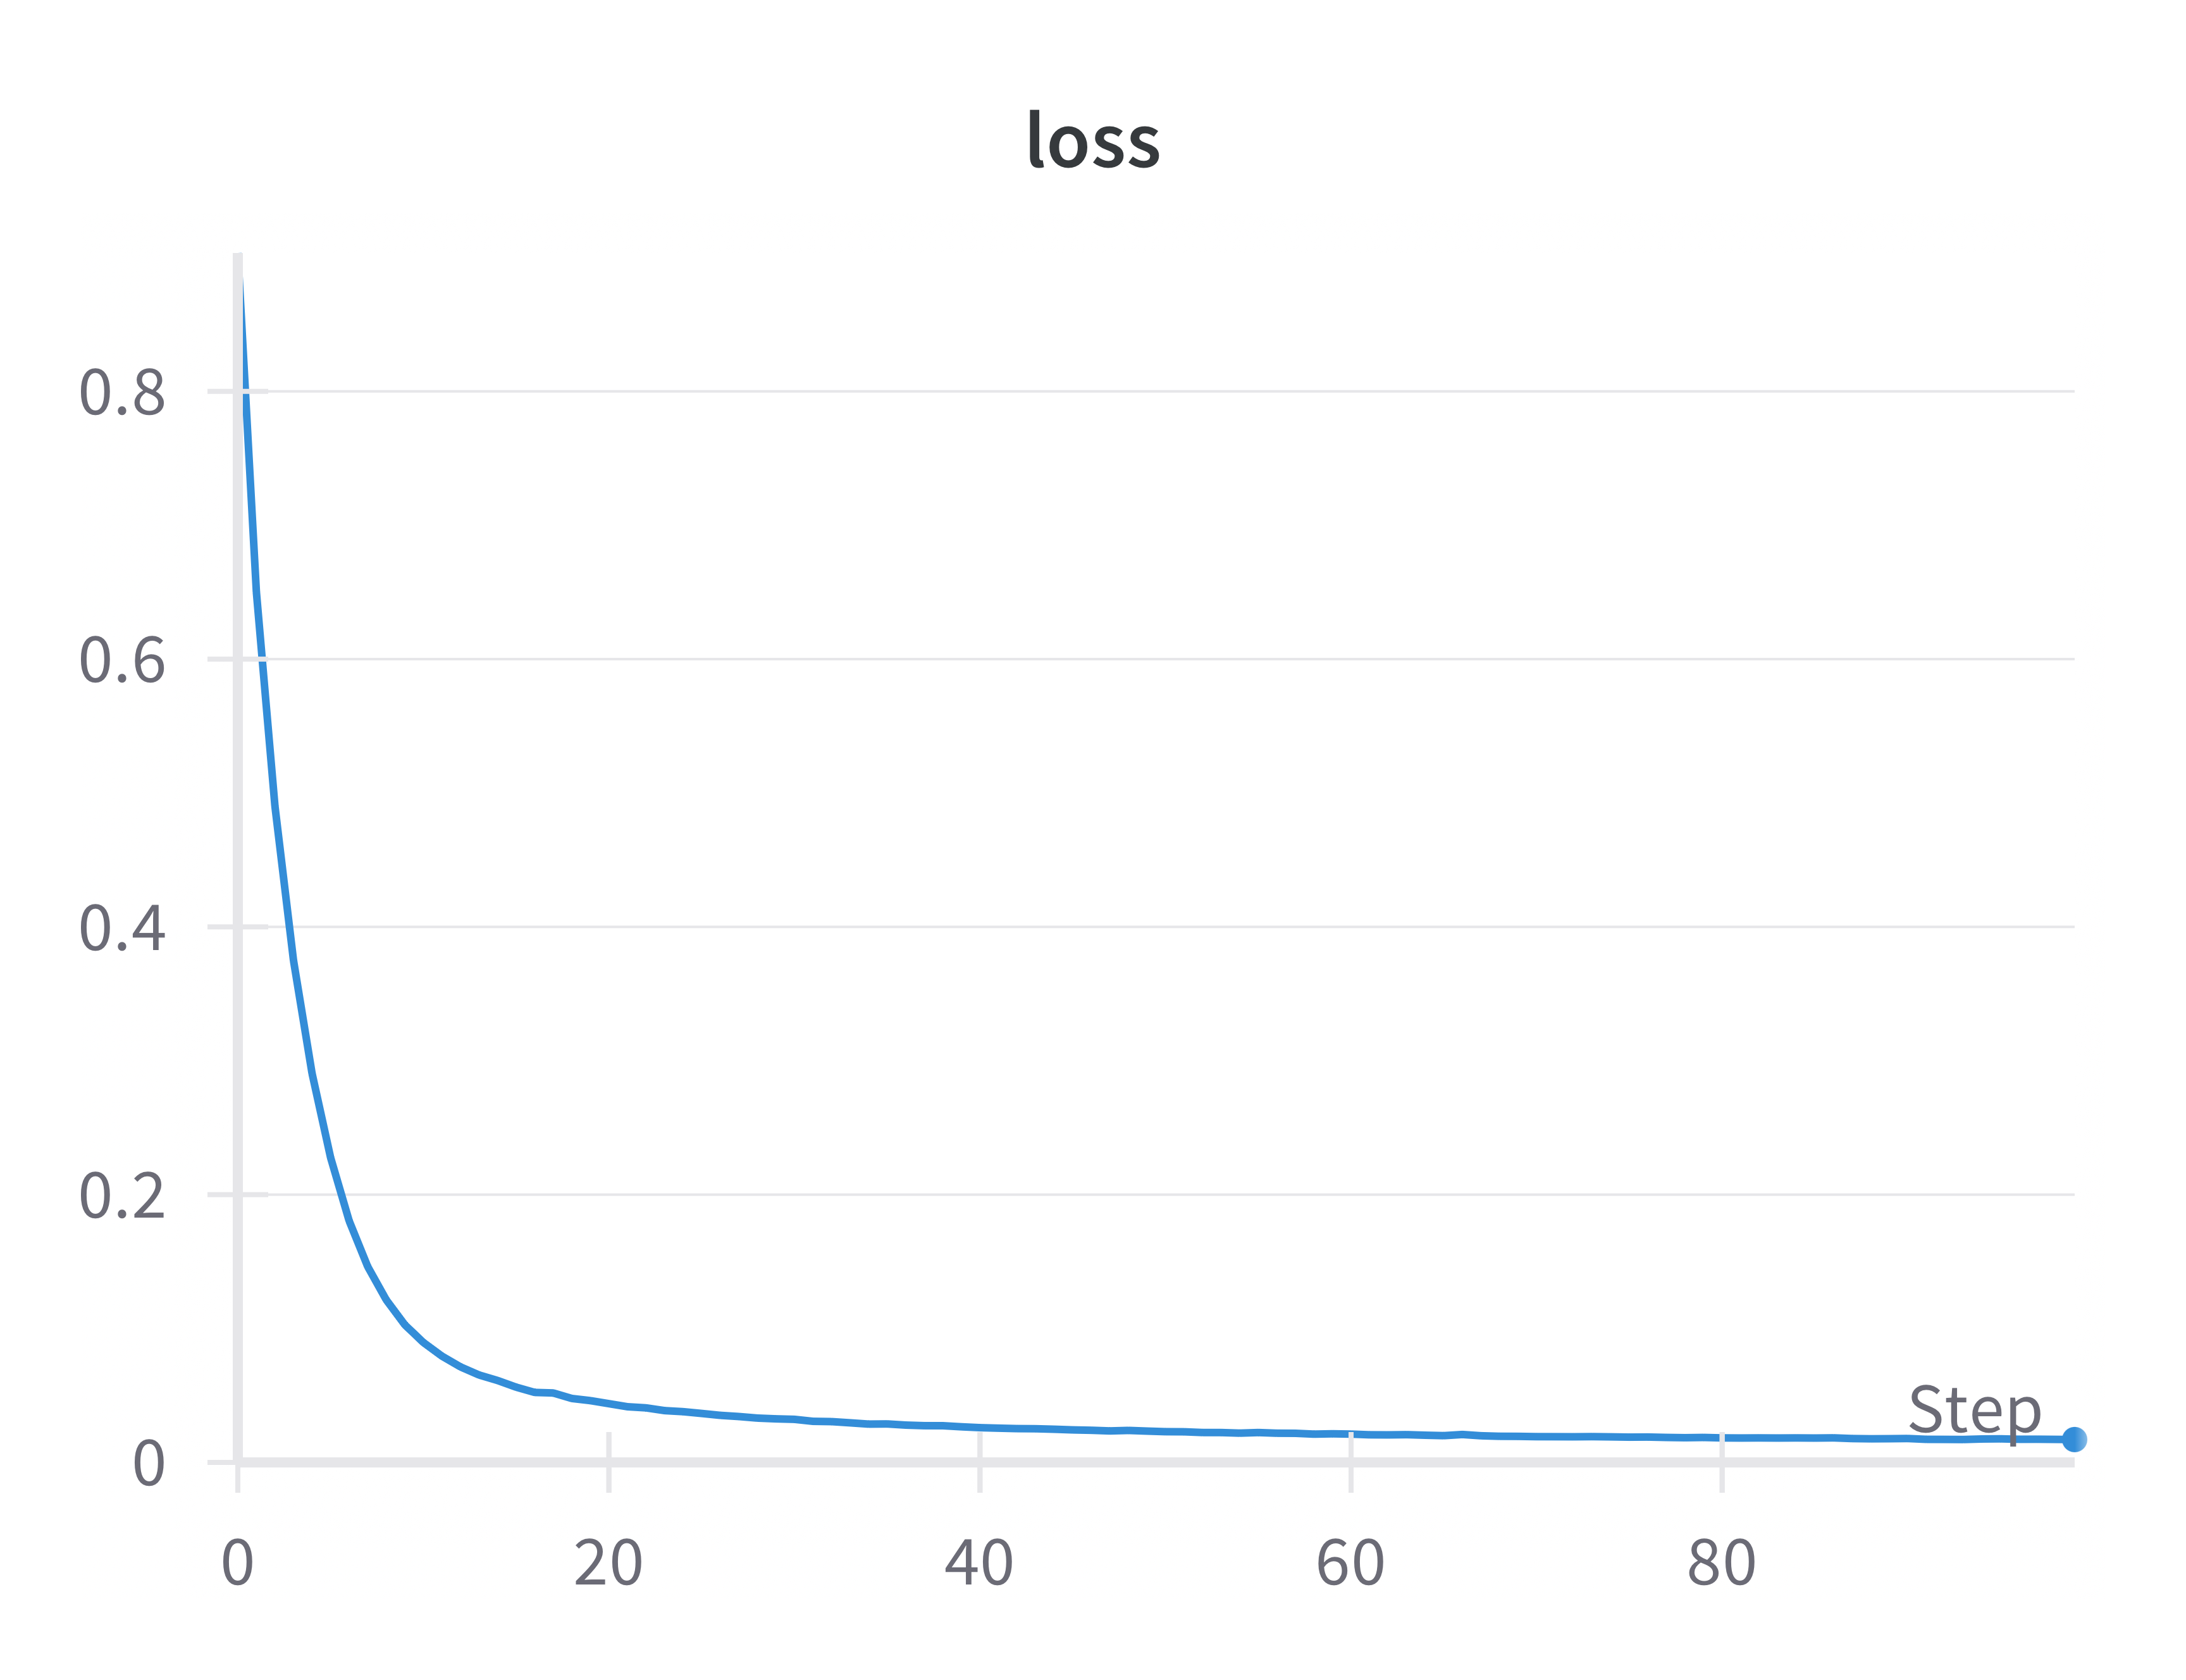
\includegraphics[width=\textwidth]{./Images/loss.png}
    \end{subfigure}
    \begin{subfigure}[b]{0.49\textwidth}
        \centering
        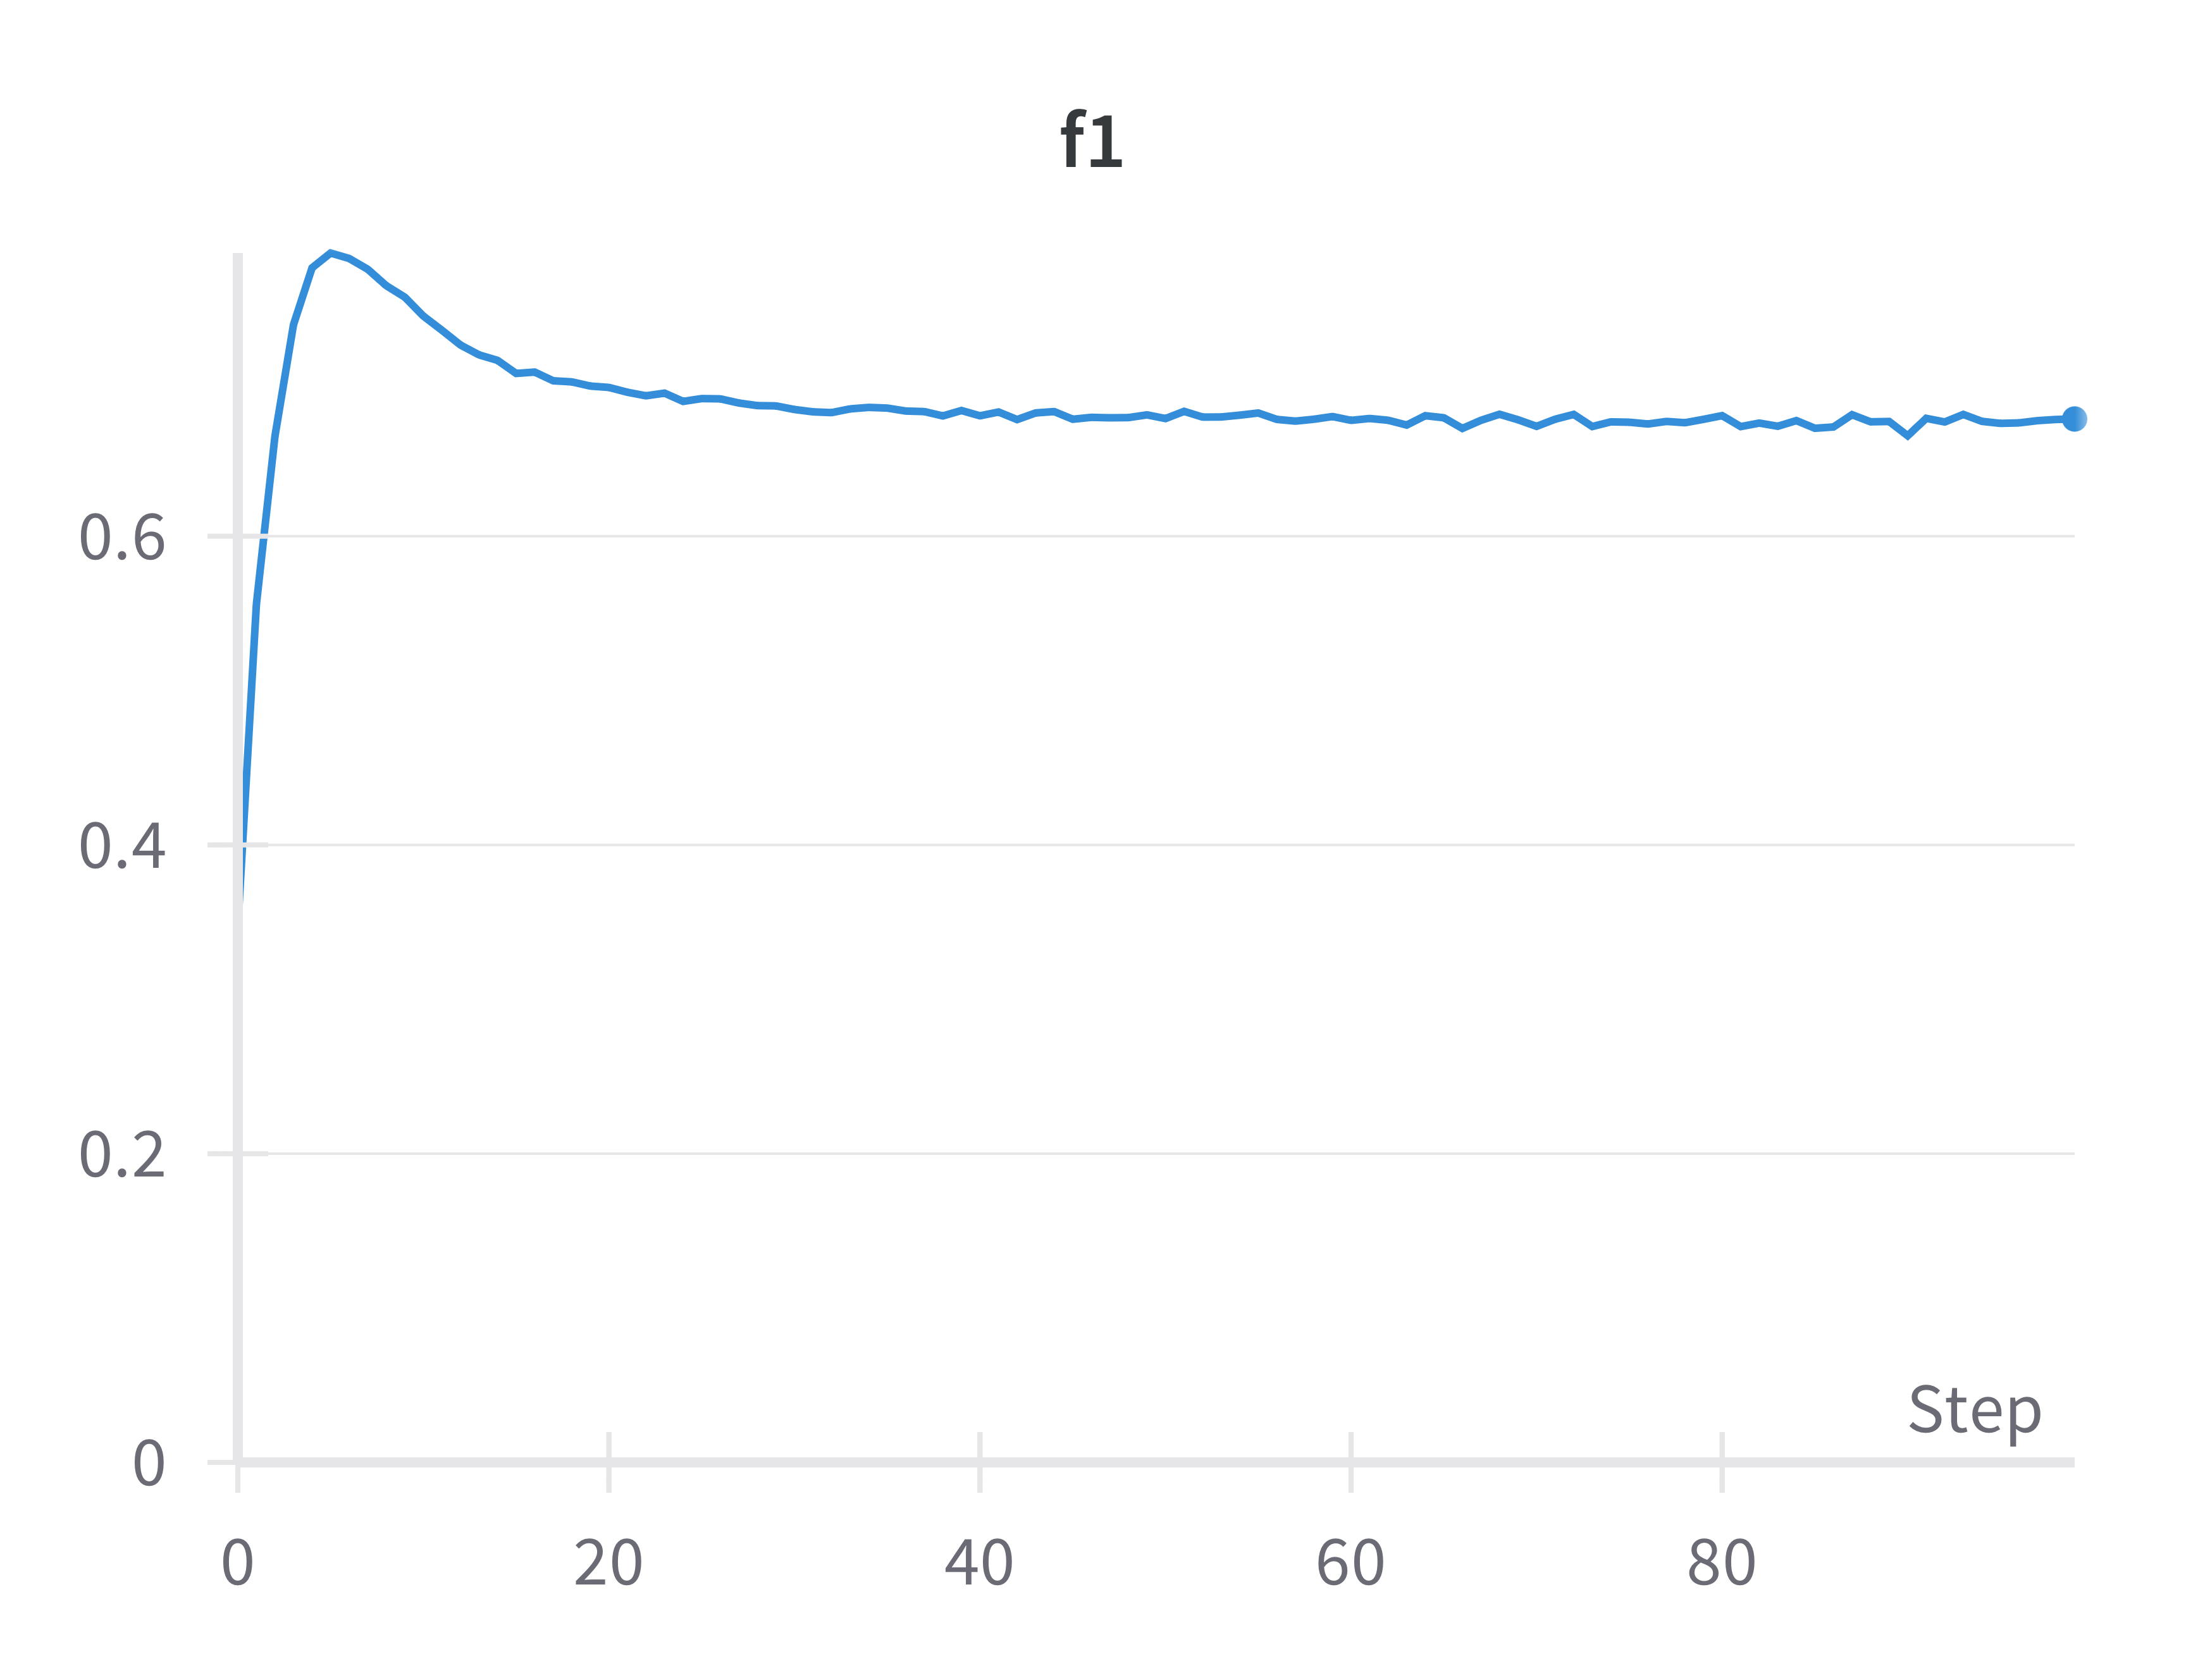
\includegraphics[width=\textwidth]{./Images/f1.png}
    \end{subfigure}
    
    \caption{The loss produced during the training process from the training dataset and the corresponding F1 score created from the validation dataset in respect to the epoch produced by W\&B}
    \label{fig:loss}
\end{figure}

\subsection*{Subtask 3}

In order to run a sweep using W\&B, we first define a new function \lstinline|train| that is called by W\&B to start a new run for the sweep according to the provided configuration.
\begin{lstlisting}
def train(config=None):        
     with wandb.init(project='x_ray_segmentation_erda', config=config):
        config = wandb.config
        
        model = smp.Unet(encoder_name='efficientnet-b0', in_channels=1, classes=1)
        model.to(device)
        metrics = {"f1": torchmetrics.classification.F1Score(task='binary', num_classes=1, average="macro")}
        loss = torch.nn.MSELoss(reduction="mean")
        
        if config.optimizer == "sgd":
            optimizer = torch.optim.SGD(model.parameters(), lr=config.learning_rate, momentum=0.9)
        elif config.optimizer == "adam":
            optimizer = torch.optim.Adam(model.parameters(), lr=config.learning_rate)
        
        train_loader = torch.utils.data.DataLoader(train_dataset, batch_size=config.batch_size, shuffle=True)
        val_loader = torch.utils.data.DataLoader(val_dataset, batch_size=config.batch_size, shuffle=False)
         
        training_loop(
            model=model,
            loss=loss,
            optimizer=optimizer,
            train_loader=train_loader,
            val_loader=val_loader,
            n_epochs=config.epochs,
            metrics_dict=metrics,
        )
\end{lstlisting}


The function consists of following parts:
\begin{enumerate}
    \item Initialize new run to track with W\&B with our provided configuration. 
    \item Define the model, metrics (which we restrict to the F1 score), and the loss function (mean squared error)
    \item Use the configuration to choose the optimizer and the batch size for the training and validation dataset. 
    \item Run \lstinline|training_loop| with this setup.
\end{enumerate}

 For the hyperparameter sweep we want to sweep over the parameters batch size, learning rate, and the choice of the optimizer with the goal to minimize the loss. This is defined in the \lstinline|sweep_config|. More details on the experimental setup will follow in Subtask 4. Finally, we initialize the sweep with the above configuration and run 16 different sweeps. 


\begin{lstlisting}
sweep_config = {
    'method': 'random',
    'metric': {'goal': 'minimize', 'name': 'loss'},
    'parameters': {
        'batch_size': {
            'distribution': 'q_log_uniform_values',
            'max': 32,
            'min': 8
        },
        'epochs': {'value': 40},
        'learning_rate': {'distribution': 'log_uniform_values',
                          'max': 0.01,
                          'min': 0.00005},
        'optimizer': {'values': ['adam', 'sgd']}
    }

sweep_id = wandb.sweep(sweep_config, project='x_ray_segmentation_erda')
wandb.agent(sweep_id, function=train, count=16)
 }
\end{lstlisting}

Figure~\ref{fig:sweep} shows the parallel coordinate plot produced by W\&B when executing the sweep.

\begin{figure}
    \centering
    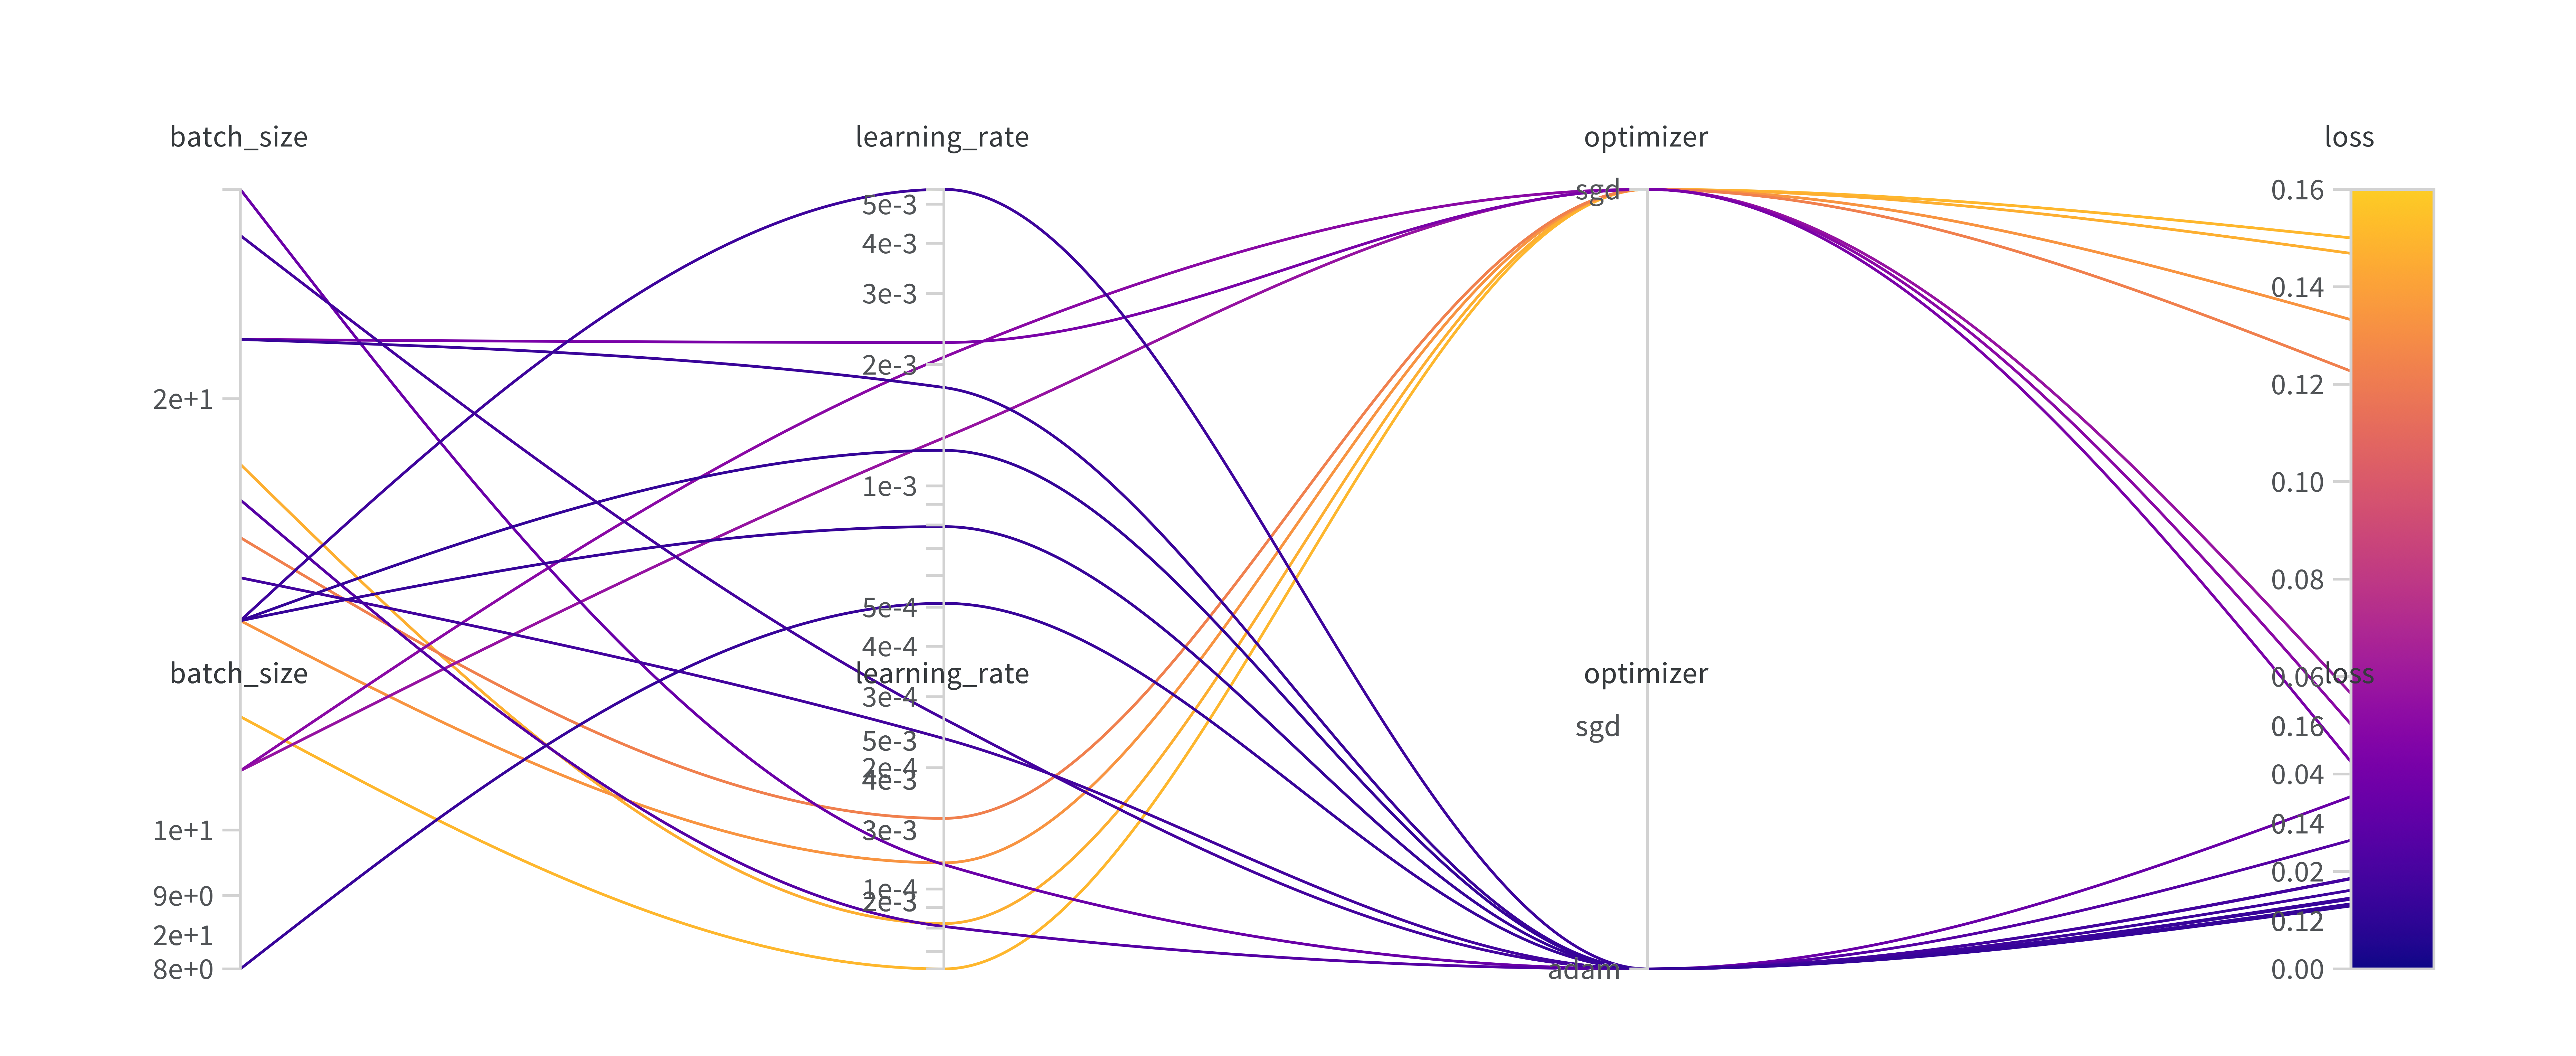
\includegraphics[width=\textwidth]{./Images/sweep.png}
    \caption{Parallel coordinate plot of sweep with 16 runs}
    \label{fig:sweep}
\end{figure}



\subsection*{Subtask 4}

For the hyperparameter sweep, we will limit the number of epochs to 40 to reduce training time. We will sweep over the parameters batch size, learning rate, and the choice of the optimizer. We aim to minimize the loss. Table~\ref{tab:sweep} presents the range of values for each parameter, plus the distribution of the values.

\begin{table}
    \centering
    \begin{tabular}{l|l|l}
        \textbf{Parameter} & \textbf{Values} & \textbf{Distribution}  \\\hline
        Batch Size & $[8,32]$ & Quantized log-uniform\\
        Learning Rate & $[0.00005, 0.01]$ & Log-Uniform \\
        Optimizer & $\{\text{Adam}, \text{SGD}\}$ & Uniform\\
    \end{tabular}
    \caption{Sweep configuration}
    \label{tab:sweep}
\end{table}

The results of the sweep are recorded by W\&B and shown in Figure~\ref{fig:sweep} with the help of a parallel coordinate plot.

What we can see right away is that the loss of the runs using Adam is lower ($< 0.04$) than runs using SGD ($> 0.04$). If we further trend that can be seen when focusing on the runs using SGD is that, in general, a lower learning rate ($<0.0002$) leads to a higher loss ($>0.12$) whereas runs with a higher learning rate ($> 0.001$) lead to a lower loss ($<0.06$). When looking at the learning rate for runs using Adam, we can see a similar trend: runs with a learning rate below $0.0002$ yield a loss less than $0.02$, runs with a learning rate above $0.0002$ yield a loss greater than $0.02$. When looking at the batch size, no clear trend can be observed.

The results suggest that the Adam optimizer in general yields better results than SGD. When it comes to learning rate, it seems to be the case that a learning rate slightly higher than $0.0002$ seems to yield better results as runs with a learning rate less than this. However, the data does not hint that the performance generally improves by simply increasing the learning rate. Above $0.0002$, the results yield very similar results. In order to draw a more concrete conclusion here, more experiments are needed. This also is the case when considering batch size, as we also do not observe any specific trend from the data.


\end{document}